\documentclass[12pt, a4paper]{article}
\usepackage{xeCJK} % Support for Chinese characters
\setCJKmainfont{Microsoft JhengHei}[
    AutoFakeBold=2.5,
    AutoFakeItalic=true
]
\setCJKmonofont{Microsoft JhengHei}
\renewcommand{\tablename}{表}
\renewcommand{\figurename}{圖}

% Packages
\usepackage{geometry}
\geometry{left=2.5cm, right=2.5cm, top=2.5cm, bottom=2.5cm}
\usepackage{amsmath}
\usepackage{amssymb}
\usepackage{graphicx}
\usepackage{booktabs}
\usepackage{array}
\usepackage{float}
\usepackage{listings}
\usepackage{xcolor}
\usepackage{hyperref}
\usepackage{longtable}
\usepackage{caption}
\usepackage{tikz}
\usetikzlibrary{positioning, arrows.meta}

% Hyperref Setup
\hypersetup{
    colorlinks=true,
    linkcolor=black,
    filecolor=blue,      
    urlcolor=blue,
    citecolor=black,
}

% Colors for listings
\definecolor{codegreen}{rgb}{0,0.6,0}
\definecolor{codegray}{rgb}{0.5,0.5,0.5}
\definecolor{codepurple}{rgb}{0.58,0,0.82}
\definecolor{backcolour}{rgb}{0.95,0.95,0.92}

\lstdefinestyle{vhdlstyle}{
    backgroundcolor=\color{backcolour},   
    commentstyle=\color{codegreen},
    keywordstyle=\color{magenta},
    numberstyle=\tiny\color{codegray},
    stringstyle=\color{codepurple},
    basicstyle=\ttfamily\footnotesize,
    breakatwhitespace=false,         
    breaklines=true,                 
    captionpos=b,                    
    keepspaces=true,                 
    numbers=left,                    
    numbersep=5pt,                  
    showspaces=false,                
    showstringspaces=false,
    showtabs=false,                  
    tabsize=2,
    frame=single,
    language=VHDL
}

\title{\textbf{2026年微處理器系統期末專案報告：\\ 四階段管線中央處理器設計與實作}}
\author{
    資訊工程學系 \\
    第 19 組 \\
    \texttt{113590051} 楊承諭（實作組，負責核心架構與程式撰寫，貢獻度 65\%） \\
    \texttt{113590017} 黃楷程（報告組，負責測資驗證與報告彙整，貢獻度 35\%）
}
\date{2026年6月26日}

\begin{document}

\maketitle

\hrule
\vspace{1.5em}

\section*{實驗基本資訊}
\begin{itemize}
    \item \textbf{實驗主題}：四階段管線中央處理器設計與實作 (4-Stage Pipeline CPU Design \& Implementation)
    \item \textbf{班級}：資訊工程學系
    \item \textbf{學號/姓名}：
    \begin{itemize}
        \item \texttt{113590051} 楊承諭 (負責核心架構與程式撰寫)
        \item \texttt{113590017} 黃楷程 (負責測資驗證與報告彙整)
    \end{itemize}
    \item \textbf{組別}：第 19 組
    \item \textbf{實驗日期}：2026年6月26日
\end{itemize}

\vspace{1.5em}
\hrule
\newpage

\section{實驗目的與專案要求}

本期末專案的目標是在 Altera DE2-115 開發板（Cyclone IV E 晶片）上，使用 \textbf{VHDL 語言}設計並實作一個\textbf{四階段管線中央處理器（4-Stage Pipeline CPU）}。本專案核心要求如下：

\begin{enumerate}
    \item \textbf{管線化設計}：所有指令的執行均須以管線（Pipeline）方式實現，包含四個階段：
    \begin{itemize}
        \item \textbf{IF (Instruction Fetch)}：讀取指撥開關的指令與資料。
        \item \textbf{ID (Instruction Decode / Register Read)}：解碼並讀取暫存器陣列，進行前饋判斷。
        \item \textbf{EXE (Execution)}：執行 ALU 運算或啟動多時序除法器。
        \item \textbf{WB (Write Back)}：將運算結果寫回暫存器檔案。
    \end{itemize}
    \item \textbf{資料衝突與前饋機制 (Data Hazard \& Forwarding)}：必須設計 Forwarding Unit，自動偵測並處理 \textbf{EXE 階段與 WB 階段的資料衝突}，使得單週期指令（LOAD, MOVE, ADD 等）在發生相依性時能夠 \textbf{Zero-Stall} 連續執行，並以綠色 LED 燈 \texttt{LEDG[0]} 即時指示衝突發生。
    \item \textbf{多時序除法器 (Multi-cycle DIV) 與管線暫停 (Stall)}：進階功能要求實作符合 Lab 7 規格的\textbf{移位相減式除法器（Restoring Division）}，對 8-bit 資料進行多時序（8 clocks）除法運算。除法執行期間管線必須正確暫停（Stall）其他階段，插入氣泡（Bubble）以防止 WB 誤寫回，並以綠色 LED 燈 \texttt{LEDG[1]} 顯示 \texttt{exe\_busy}（管線暫停狀態）。此外需具備\textbf{除以零防錯與 Bypass 機制}，若除數為 0 則不進行 8 週期 Stall，直接輸出錯誤碼 \texttt{0xFF}。
    \item \textbf{硬體周邊與顯示驅動}：
    \begin{itemize}
        \item 使用七段顯示器即時顯示 Rs、Rt 暫存器之數值（十六進制 \texttt{00}\textasciitilde\texttt{FF}）。
        \item 使用七段顯示器分別顯示當前的輸入指令 Opcode、IF/ID管線暫存器 Opcode，以及 ID/EXE 管線暫存器 Opcode。
        \item 使用紅色 LED \texttt{LEDR[7:0]} 顯示當前指撥開關輸入的 8 位元立即值（Data）。
    \end{itemize}
\end{enumerate}

\section{核心硬體架構與規格設計}

\subsection{微架構管線暫存器定義}

為了在硬體上實現 4-stage 管線，我們定義了三組管線暫存器（Pipeline Registers）來劃分各階段邊界，並在每個 Clock 正緣（即手動按鍵 \texttt{KEY[0]} 被按下並釋放時）同步更新：

\begin{itemize}
    \item \textbf{IF/ID 暫存器}：鎖存自 \texttt{SW[15:0]} 擷取的指令欄位。
    \begin{itemize}
        \item \texttt{IFID\_opcode} (4-bit)：存儲當前指令操作碼。
        \item \texttt{IFID\_rs\_id} (2-bit)：存儲目標暫存器選擇子。
        \item \texttt{IFID\_rt\_id} (2-bit)：存儲來源暫存器選擇子。
        \item \texttt{IFID\_data} (8-bit)：存儲 8 位元立即值。
    \end{itemize}
    \item \textbf{ID/EXE 暫存器}：鎖存解碼完成、暫存器讀取（或前饋後）的運算元。
    \begin{itemize}
        \item \texttt{IDEXE\_opcode} (4-bit)
        \item \texttt{IDEXE\_rs\_id} (2-bit)
        \item \texttt{IDEXE\_rs\_val} (8-bit)：前饋或暫存器檔案讀出的 Rs 數值。
        \item \texttt{IDEXE\_rt\_id} (2-bit)
        \item \texttt{IDEXE\_rt\_val} (8-bit)：前饋或暫存器檔案讀出的 Rt 數值。
        \item \texttt{IDEXE\_data} (8-bit)：傳遞給 EXE 階段的 LOAD 立即值。
    \end{itemize}
    \item \textbf{EXE/WB 暫存器}：鎖存 EXE 階段 ALU 或除法狀態機的最終結果，準備在 WB 階段寫回。
    \begin{itemize}
        \item \texttt{EXEWB\_opcode} (4-bit)
        \item \texttt{EXEWB\_rs\_id} (2-bit)：寫回目標暫存器 ID。
        \item \texttt{EXEWB\_result} (8-bit)：寫回資料。
    \end{itemize}
\end{itemize}

\subsection{資料前饋單元 (Forwarding Unit) 設計邏輯}

當後續指令需要讀取前序指令尚未寫回暫存器檔案（Register File）的最新結果時，會產生資料衝突（Data Hazard）。本處理器設計了完整的前饋機制，其邏輯架構如圖 \ref{fig:forwarding_unit} 所示：

\begin{figure}[H]
\centering
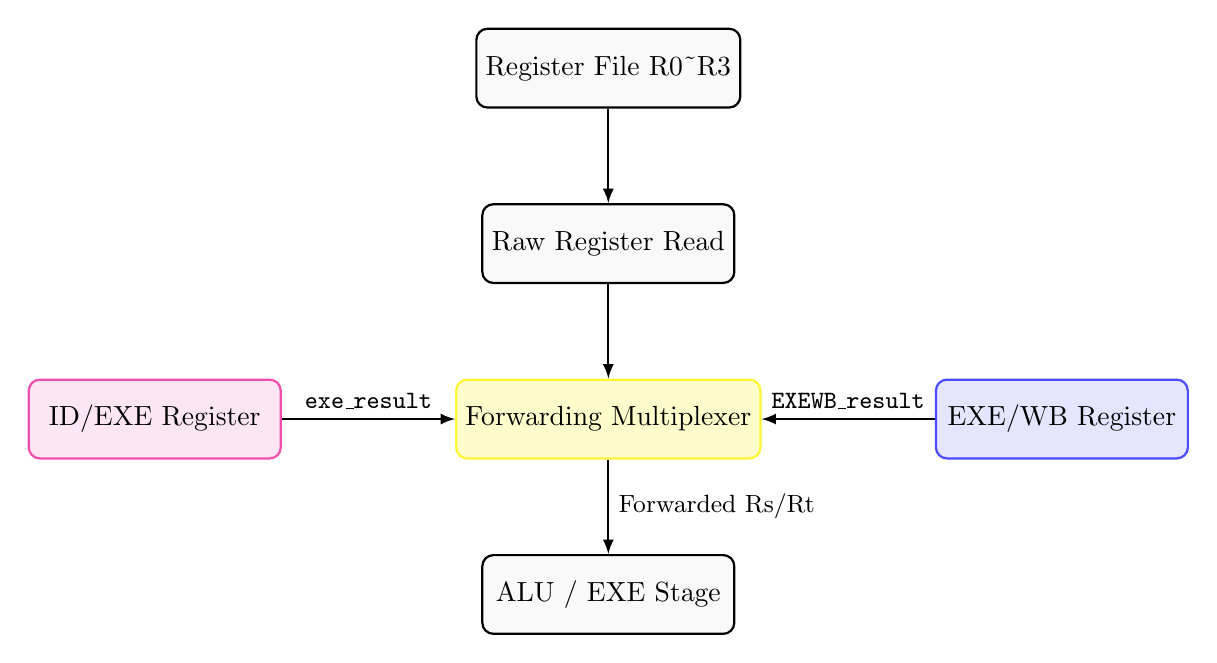
\begin{tikzpicture}[
    node distance=1.2cm and 1cm,
    box/.style={draw, rectangle, rounded corners, minimum width=3.2cm, minimum height=1cm, align=center, thick, fill=gray!5},
    pinkbox/.style={box, fill=magenta!10, draw=magenta!70},
    bluebox/.style={box, fill=blue!10, draw=blue!70},
    yellowbox/.style={box, fill=yellow!20, draw=yellow!80},
    arrow/.style={-latex, thick}
]
    \node[box] (regfile) {Register File R0\textasciitilde R3};
    \node[box, below=of regfile] (rawread) {Raw Register Read};
    \node[yellowbox, below=of rawread] (fwdmux) {Forwarding Multiplexer};
    \node[pinkbox, left=2.2cm of fwdmux] (exereg) {ID/EXE Register};
    \node[bluebox, right=2.2cm of fwdmux] (wbreg) {EXE/WB Register};
    \node[box, below=of fwdmux] (alu) {ALU / EXE Stage};

    \draw[arrow] (regfile) -- (rawread);
    \draw[arrow] (rawread) -- (fwdmux);
    \draw[arrow] (exereg) -- node[above, font=\small] {\texttt{exe\_result}} (fwdmux);
    \draw[arrow] (wbreg) -- node[above, font=\small] {\texttt{EXEWB\_result}} (fwdmux);
    \draw[arrow] (fwdmux) -- node[right, font=\small] {Forwarded Rs/Rt} (alu);
\end{tikzpicture}
\caption{前饋單元 (Forwarding Unit) 邏輯架構圖}
\label{fig:forwarding_unit}
\end{figure}

\begin{itemize}
    \item \textbf{衝突偵測邏輯}：
    我們需要確認當前處於 ID 階段的指令是否確實需要讀取 \texttt{Rs} 或 \texttt{Rt} 暫存器。若指令為 \texttt{LOAD}（僅寫入 \texttt{Rs}）或 \texttt{NOP}，則不應參與前饋判定。
    \begin{itemize}
        \item \texttt{reads\_rs} 成立條件：指令為 \texttt{ADD}, \texttt{AND}, \texttt{SLT}, \texttt{SUB(A-B)}, \texttt{NOR}, \texttt{SUB(B-A)}, \texttt{DIV}。
        \item \texttt{reads\_rt} 成立條件：指令為上述運算指令，或 \texttt{MOVE}（讀取 \texttt{Rt} 複製到 \texttt{Rs}）。
    \end{itemize}

    \item \textbf{EXE 階段衝突前饋 (EXE Forwarding)}：
    若 ID 階段讀取的暫存器與處於 EXE 階段的指令寫回暫存器相符，且 EXE 階段指令有效，則直接前饋 \texttt{exe\_result}。
    \[
    \text{fwd\_rs\_exe} = \text{reads\_rs} \land \text{IDEXE\_valid} \land (\text{IDEXE\_opcode} \neq \text{NOP}) \land (\text{IDEXE\_rs\_id} = \text{IFID\_rs\_id})
    \]
    \[
    \text{fwd\_rt\_exe} = \text{reads\_rt} \land \text{IDEXE\_valid} \land (\text{IDEXE\_opcode} \neq \text{NOP}) \land (\text{IDEXE\_rs\_id} = \text{IFID\_rt\_id})
    \]

    \item \textbf{WB 階段衝突前饋 (WB Forwarding)}：
    若 ID 階段讀取的暫存器與處於 WB 階段的指令寫回暫存器相符，且 WB 階段指令有效，且未被 EXE 階段的前饋（較新的值）覆蓋，則前饋 \texttt{EXEWB\_result}。
    \[
    \text{fwd\_rs\_wb} = \text{reads\_rs} \land \text{EXEWB\_valid} \land (\text{EXEWB\_opcode} \neq \text{NOP}) \land (\text{EXEWB\_rs\_id} = \text{IFID\_rs\_id}) \land \neg\text{fwd\_rs\_exe}
    \]
    \[
    \text{fwd\_rt\_wb} = \text{reads\_rt} \land \text{EXEWB\_valid} \land (\text{EXEWB\_opcode} \neq \text{NOP}) \land (\text{EXEWB\_rs\_id} = \text{IFID\_rt\_id}) \land \neg\text{fwd\_rt\_exe}
    \]

    \item \textbf{衝突指示燈}：
    若對任何一個有效指令啟動了前饋機制（\texttt{fwd\_rs\_exe}、\texttt{fwd\_rs\_wb}、\texttt{fwd\_rt\_exe} 或 \texttt{fwd\_rt\_wb} 為真），則綠色 LED \texttt{LEDG[0]} 會即時亮起。
\end{itemize}

\subsection{多時序除法狀態機與管線 Stall 機制}

除法指令 \texttt{DIV Rs, Rt} 需要多個 Clock 進行移位相減運算，無法在單個時脈週期內完成。我們在 EXE 階段設計了一個 Restoring Division 有限狀態機（FSM），其狀態移轉如圖 \ref{fig:div_fsm} 所示：

\begin{figure}[H]
\centering
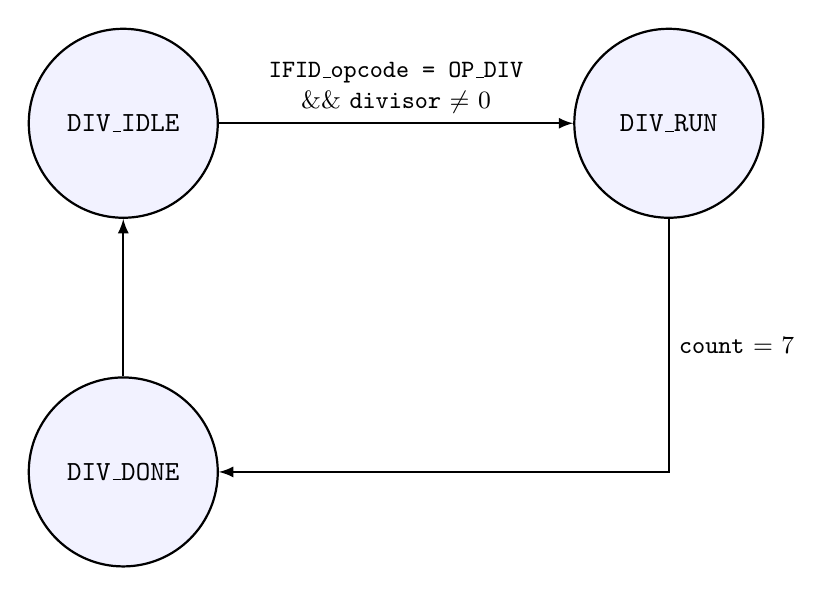
\begin{tikzpicture}[
    >=latex,
    node distance=2.5cm,
    state/.style={draw, circle, minimum size=2.4cm, align=center, thick, fill=blue!5},
    arrow/.style={->, thick}
]
    \node[state] (idle) {\texttt{DIV\_IDLE}};
    \node[state, right=4.5cm of idle] (run) {\texttt{DIV\_RUN}};
    \node[state, below=2cm of idle] (done) {\texttt{DIV\_DONE}};

    \draw[arrow] (idle) -- node[above, align=center, font=\small] {
        \texttt{IFID\_opcode = OP\_DIV} \\
        \&\& \texttt{divisor} $\neq$ 0
    } (run);
    \draw[arrow] (run) |- node[right, pos=0.25, font=\small] {\texttt{count} = 7} (done);
    \draw[arrow] (done) -- (idle);
\end{tikzpicture}
\caption{多時序除法狀態機 (FSM) 狀態移轉圖}
\label{fig:div_fsm}
\end{figure}

\begin{itemize}
    \item \textbf{DIV\_IDLE}：空閒狀態。當偵測到即將進入 ID/EXE 暫存器的指令為 \texttt{DIV}，且除數不為 0 時，於時脈正緣載入被除數 \texttt{Rs\_val\_fwd} 至 \texttt{div\_dividend}，除數 \texttt{Rt\_val\_fwd} 至 \texttt{div\_divisor}，並跳轉至 \texttt{DIV\_RUN}，計數器 \texttt{div\_count} 歸零。
    \item \textbf{DIV\_RUN}：執行 8-bit 恢復除法演算法。每個時脈執行以下步驟：
    \begin{enumerate}
        \item 將餘數暫存器 \texttt{div\_rem} 左移 1 位，並讀入被除數 \texttt{div\_dividend} 的最高位元。
        \item 比較此暫時值是否大於等於除數 \texttt{div\_divisor}。
        \item 若大於等於，則 \texttt{div\_rem} 扣除 \texttt{div\_divisor}，且商數 \texttt{div\_quot} 的對應位元置為 \texttt{1}。
        \item 若小於，則 \texttt{div\_rem} 保持原值，商數該位元保持 \texttt{0}。
        \item \texttt{div\_count} 遞增，直到第 8 個時脈（計數值為 7）計算完畢後跳轉至 \texttt{DIV\_DONE}。
    \end{enumerate}
    \item \textbf{DIV\_DONE}：除法運算結束。在此狀態下，商數 \texttt{div\_quot} 輸出至 \texttt{exe\_result}，狀態機在下一個時脈回到 \texttt{DIV\_IDLE}。
\end{itemize}

\subsubsection{管線暫停 (Stall) 與氣泡插入 (Bubble) 控制：}

當狀態機處於 \texttt{DIV\_RUN} 狀態時，\texttt{stall} 訊號為 \texttt{1}。管線控制器在此期間進行以下時序操作：

\begin{enumerate}
    \item \textbf{凍結上游階段}：不對 \texttt{IF/ID} 和 \texttt{ID/EXE} 管線暫存器進行更新。此時，指撥開關的輸入與解碼出的暫存器值保持鎖定。
    \item \textbf{插入氣泡（Bubble）}：為了防止 EXE/WB 暫存器在管線暫停期間重複寫入無效資料，管線暫存器 \texttt{EXEWB} 會被強制寫入 \texttt{OP\_NOP} (1111) 且 \texttt{valid} 設為 \texttt{0}。這代表將一個「氣泡」送入 WB 階段，避免管線寫回暫存器。
    \item \textbf{除法結束推進}：當狀態機進入 \texttt{DIV\_DONE}，\texttt{stall} 降為 \texttt{0}，\texttt{exe\_result} 順利傳遞給 \texttt{EXE/WB}，管線恢復正常推進。
\end{enumerate}

\subsubsection{除以零防錯 Bypass：}

若在 \texttt{DIV\_IDLE} 狀態下偵測到除數（\texttt{Rt\_val\_fwd}）為 \texttt{0}，狀態機將\textbf{直接進入 \texttt{DIV\_DONE} 狀態}，並將結果 \texttt{div\_quot} 設為錯誤碼 \texttt{0xFF}。因為不經過 \texttt{DIV\_RUN}，\texttt{stall} 訊號保持為 \texttt{0}。這使得除以零指令能像單週期指令一樣 \textbf{Zero-Stall} 快速流過管線，並在 WB 階段正確將 \texttt{0xFF} 寫入 Rs，完美符合專案的防錯 Bypass要求。

\section{硬體週邊配置與腳位對照表}

本專案在 Quartus II 軟體中將實體 I/O 腳位與 DE2-115 開發板進行了完全綁定。以下為腳位配置對照表：

\subsection{指撥開關（輸入）與按鈕時脈}

\begin{table}[H]
    \centering
    \caption{輸入週邊與腳位對照表}
    \label{tab:input_pin}
    \begin{tabular}{@{}llp{8cm}l@{}}
        \toprule
        \textbf{埠名稱 (Port)} & \textbf{位元寬度} & \textbf{對應板載硬體週邊 (Component)} & \textbf{FPGA 晶片腳位 (Pin)} \\ \midrule
        \texttt{KEY[0]}              & 1 & 系統手動時脈輸入（手動按鍵，按下觸發）  & \texttt{PIN\_M23} \\
        \texttt{SW[7]} \textasciitilde\ \texttt{SW[0]}   & 8 & 8位元立即值資料輸入（Data / Immediate） & \texttt{PIN\_AB26} \textasciitilde\ \texttt{PIN\_AB28} 等 \\
        \texttt{SW[11]} \textasciitilde\ \texttt{SW[8]}  & 4 & 4位元指令操作碼輸入（Opcode）           & \texttt{PIN\_AB24}, \texttt{PIN\_AC24}, \texttt{PIN\_AB25}, \texttt{PIN\_AC25} \\
        \texttt{SW[13]} \textasciitilde\ \texttt{SW[12]} & 2 & 目標暫存器選擇子（Rs register select）  & \texttt{PIN\_AA24}, \texttt{PIN\_AB23} \\
        \texttt{SW[15]} \textasciitilde\ \texttt{SW[14]} & 2 & 來源暫存器選擇子（Rt register select）  & \texttt{PIN\_AA22}, \texttt{PIN\_AA23} \\ \bottomrule
    \end{tabular}
\end{table}

\subsection{七段顯示器與 LED 燈（輸出）}

\begin{table}[H]
    \centering
    \caption{輸出週邊與腳位對照表}
    \label{tab:output_pin}
    \begin{tabular}{@{}llp{8cm}l@{}}
        \toprule
        \textbf{埠名稱 (Port)} & \textbf{位元寬度} & \textbf{對應板載硬體週邊 (Component)} & \textbf{FPGA 晶片腳位 (Pin)} \\ \midrule
        \texttt{HEX1}, \texttt{HEX0} & 14 & Rs 暫存器數值顯示（HEX1十位、HEX0個位，範圍\texttt{00}\textasciitilde\texttt{FF}） & \texttt{PIN\_M24}\textasciitilde\texttt{PIN\_U24}, \texttt{PIN\_G18}\textasciitilde\texttt{PIN\_H22} \\
        \texttt{HEX3}, \texttt{HEX2} & 14 & Rt 暫存器數值顯示（HEX3十位、HEX2個位，範圍\texttt{00}\textasciitilde\texttt{FF}） & \texttt{PIN\_V21}\textasciitilde\texttt{PIN\_Y19}, \texttt{PIN\_AA25}\textasciitilde\texttt{PIN\_W28} \\
        \texttt{HEX4}           & 7  & IF/ID 管線暫存器中鎖存之指令 Opcode (顯示\texttt{0}\textasciitilde\texttt{F})      & \texttt{PIN\_AB19} \textasciitilde\ \texttt{PIN\_AE18} \\
        \texttt{HEX5}           & 7  & Live 即時輸入之指令 Opcode（隨 SW[11:8] 即時變動）         & \texttt{PIN\_AD18} \textasciitilde\ \texttt{PIN\_AH18} \\
        \texttt{HEX6}           & 7  & ID/EXE 管線暫存器中鎖存之指令 Opcode (顯示\texttt{0}\textasciitilde\texttt{F})     & \texttt{PIN\_AA17} \textasciitilde\ \texttt{PIN\_AC17} \\
        \texttt{LEDR[7:0]}      & 8  & 紅色 LED，即時顯示例立值資料數值（\texttt{SW[7:0]}）            & \texttt{PIN\_G19} \textasciitilde\ \texttt{PIN\_H19} 等 \\
        \texttt{LEDG[0]}        & 1  & 綠色 LED，資料衝突與前饋指示器（Hazard Detected）          & \texttt{PIN\_E21} \\
        \texttt{LEDG[1]}        & 1  & 綠色 LED，除法器 Busy/管線暫停指示器（Exe Busy）           & \texttt{PIN\_E22} \\ \bottomrule
    \end{tabular}
\end{table}

\section{VHDL 原始碼架構分析}

本系統完全實作於單個 VHDL 檔案 \href{file:///home/chengyu/\%E6%A1%8C%E9%9D%A2/Microcomputer_System/Finial_Project/pipiline/Pipeline_CPU.vhd}{Pipeline\_CPU.vhd} 中，程式結構清晰，劃分為模組化的組合邏輯電路與同步時序電路：

\subsection*{1. 實體定義與 7 段解碼邏輯}

\texttt{to\_7seg} 函式將 4-bit 的十六進制數值解碼為主動低電位（Active-Low）的七段顯示器段碼。例如，\texttt{0000} 被解碼為 \texttt{"1000000"}（顯示 0），\texttt{1111} 解碼為 \texttt{"0001110"}（顯示 F）。這確保了暫存器值與 Opcode 在開發板上呈現清晰的十六進制。

\subsection{資料路徑前饋邏輯 (VHDL組合邏輯程式片段)}

為了確保 Zero-Stall 前饋，暫存器檔案的讀取與 Forwarding 邏輯必須是組合邏輯（即時運算）。
程式中透過以下敏感度清單 Process，動態分析目前 \texttt{IF/ID} 指令是否與下游暫存器發生 Hazard：

\begin{lstlisting}[style=vhdlstyle, caption={組合邏輯前饋與 conflict 偵測程式片段}, label={lst:forwarding_logic}]
-- 節錄自 Pipeline_CPU.vhd (組合邏輯前饋單元)
process(IFID_rs_id, IFID_rt_id, IFID_valid, IFID_opcode,
        IDEXE_rs_id, IDEXE_valid, IDEXE_opcode,
        EXEWB_rs_id, EXEWB_valid, EXEWB_opcode,
        Rs_val_raw, Rt_val_raw, exe_result, EXEWB_result)
...
begin
    -- 1. 判斷當前指令是否讀取暫存器 Rs, Rt (以屏蔽 LOAD / NOP 的誤判)
    if IFID_opcode = OP_ADD or ... then
        reads_rs_v := true; reads_rt_v := true;
    elsif IFID_opcode = OP_MOVE then
        reads_rs_v := false; reads_rt_v := true;
    else
        reads_rs_v := false; reads_rt_v := false;
    end if;

    -- 2. EXE Forwarding 偵測 (優先級最高，從 EXE 階段直接拉回)
    fwd_rs_exe := reads_rs_v and (IDEXE_valid = '1') and (IDEXE_opcode /= OP_NOP) and (IDEXE_rs_id = IFID_rs_id);
    fwd_rt_exe := reads_rt_v and (IDEXE_valid = '1') and (IDEXE_opcode /= OP_NOP) and (IDEXE_rs_id = IFID_rt_id);

    -- 3. WB Forwarding 偵測 (優先級次之，從 WB 寫回暫存器拉回)
    fwd_rs_wb := reads_rs_v and (EXEWB_valid = '1') and (EXEWB_opcode /= OP_NOP) and (EXEWB_rs_id = IFID_rs_id) and (not fwd_rs_exe);
    fwd_rt_wb := reads_rt_v and (EXEWB_valid = '1') and (EXEWB_opcode /= OP_NOP) and (EXEWB_rs_id = IFID_rt_id) and (not fwd_rt_exe);

    -- 4. 前饋多路選擇器 (Mux)
    if fwd_rs_exe then Rs_val_fwd <= exe_result;
    elsif fwd_rs_wb then Rs_val_fwd <= EXEWB_result;
    else Rs_val_fwd <= Rs_val_raw;
    end if;
    ...
\end{lstlisting}

這種設計使得暫存器讀取端能夠在時脈正緣來臨前，就經由前饋路徑獲得最即時、正確的資料。

\subsection{同步管線暫停與氣泡插入 (VHDL時序邏輯程式片段)}

多時序除法 FSM 在同步 Process 中更新狀態。在 \texttt{DIV\_RUN} 狀態下，\texttt{stall} 訊號為真，這會阻止其餘管線暫存器的前進：

\begin{lstlisting}[style=vhdlstyle, caption={時序邏輯中 Stall 氣泡插入與除法器推進程式片段}, label={lst:stall_logic}]
-- 節錄自 Pipeline_CPU.vhd (同步時序 Process 中的 Stall 分支)
if stall = '0' then
    -- 正常管線推進：WB 寫回暫存器、管線暫存器向前推進
    if EXEWB_valid = '1' and EXEWB_opcode /= OP_NOP then
        -- 寫回暫存器檔案
        case EXEWB_rs_id is ...
    end if;
    EXEWB_opcode <= IDEXE_opcode;
    IDEXE_opcode <= IFID_opcode;
    IFID_opcode  <= curr_opcode;
    ...
else
    -- 管線暫停 (DIV Stall)
    -- 1. WB 階段仍處理寫回 (第一週期完成前序指令，後續週期為氣泡)
    if EXEWB_valid = '1' and EXEWB_opcode /= OP_NOP then
        case EXEWB_rs_id is ...
    end if;
    -- 2. 插入氣泡 (Bubble) 進入 EXE/WB 暫存器
    EXEWB_opcode <= OP_NOP;
    EXEWB_valid  <= '0';
    -- 3. IFID 與 IDEXE 保持原值 (鎖定)
    -- 4. 僅除法器狀態機往前推進
    if div_state = DIV_RUN then
        bit_pos  := 7 - div_count;
        temp_rem := div_rem(6 downto 0) & div_dividend(bit_pos);
        if temp_rem >= div_divisor then
            div_rem <= temp_rem - div_divisor;
            div_quot(bit_pos) <= '1';
        else
            div_rem <= temp_rem;
        end if;
        ...
\end{lstlisting}

此結構精確實現了管線氣泡插入技術（Pipeline Bubbling），在硬體層面上消除了因除法延遲導致的多重寫回衝突。

\section{測試資料與板載硬體驗證}

我們設計了 \textbf{5 組代表性測試情境}，完整覆蓋了基本運算、EXE 衝突前饋、EXE 與 WB 同時衝突前饋、多時序除法暫停，以及除以零 Bypass 功能。以下為詳細時序與硬體狀態分析：

\subsection{測資 1：基本暫存器載入與算術運算（無 Hazard）}

\begin{itemize}
    \item \textbf{目的}：驗證管線在無衝突狀態下的基本流動與運算正確性。
    \item \textbf{指令時序序列}：
    \begin{enumerate}
        \item \texttt{Cycle 1}: \texttt{LOAD R1, 0x05} (R1 載入 5) --- \texttt{SW = 0x1005}
        \item \texttt{Cycle 2}: \texttt{LOAD R2, 0x07} (R2 載入 7) --- \texttt{SW = 0x2007}
        \item \texttt{Cycle 3}: \texttt{NOP} (空指令) --- \texttt{SW = 0x0F00}
        \item \texttt{Cycle 4}: \texttt{NOP} (空指令) --- \texttt{SW = 0x0F00}
        \item \texttt{Cycle 5}: \texttt{ADD R1, R2} (R1 \(\Leftarrow\) R1 + R2 = 12) --- \texttt{SW = 0x9200}
        \item \texttt{Cycle 6\textasciitilde 8}: 持續輸入 \texttt{NOP} (\texttt{SW = 0x0F00}) 以排空管線。
    \end{enumerate}
    \item \textbf{預期與實測結果}：
    \begin{itemize}
        \item 在 \texttt{Cycle 4} 結束後，暫存器 \texttt{R1} 的寫回完成。此時撥碼開關設定 Rs 選擇 \texttt{R1}，七段顯示器 \texttt{HEX1/0} 靜態顯示 \texttt{05}，Rt 選擇 \texttt{R2} 時 \texttt{HEX3/2} 顯示 \texttt{07}。
        \item 在 \texttt{Cycle 8} 結束後，\texttt{ADD} 指令執行並寫回完畢。\texttt{HEX1/0} 正確顯示結果 \texttt{0C} (十六進制 12)。
        \item 整個過程中，綠色 LED \texttt{LEDG[0]} (Hazard) 保持熄滅。
    \end{itemize}
\end{itemize}

\subsection{測資 2：EXE 階段資料衝突與前饋 (EXE Forwarding)}

\begin{itemize}
    \item \textbf{目的}：驗證當下一道指令需要使用「前一次運算（尚在 EXE\section{實驗心得與深度思考}

本次期末專案將原本 Lab 9 的單週期（Single-cycle）多功能 CPU 重構為四階段管線（Pipeline）架構，對我們小組而言是一次極具挑戰性且收穫豐富的實作過程。在整個設計與驗證的過程中，我們在「微架構邏輯設計」與「板載硬體驗證」兩個層面進行了深度的合作與思考：

\begin{enumerate}
    \item \textbf{管線化資料衝突與前饋機制之挑戰}：
    在單週期架構中，ALU 的運算結果是在同一個時脈週期內直接寫回暫存器。但在管線架構下，當前序指令為寫入暫存器的指令（如 \texttt{LOAD}），而緊接著的後續指令（如 \texttt{ADD}）需要讀取該暫存器時，就會產生資料衝突（Data Hazard）。
    為了在不使用暫停（Stall）的情況下達成 Zero-Stall 連續執行，我們設計了資料前饋單元（Forwarding Unit），藉由比對執行（EXE）與寫回（WB）階段的目標暫存器，將資料「直接從流水線暫存器中拉回」解碼端。
    
    在實作與偵錯過程中，我們遇到了綠色 LED \texttt{LEDG[0]} (Hazard) 持續亮起的 Bug。經 Trace 程式碼發現，這是因為 \texttt{LOAD} 指令的目標暫存器與先前的空指令 \texttt{NOP} 產生了虛假比對。我們隨即重寫了前饋判定邏輯，引入 \texttt{reads\_rs} 與 \texttt{reads\_rt} 這兩個控制訊號，以明確篩選出解碼指令是否「確實需要讀取該暫存器」，順利解決了這個 Bug。
    
    在測試與驗證端，我們也深刻感受到管線深度對時序的影響。例如在測資 1（無 Hazard 基本運算）中，為了能清晰觀察到暫存器的數值寫入與即時顯示，我們必須在 \texttt{LOAD} 後手動插入兩個 \texttt{NOP}。這是因為在四階段管線中，指令從讀入指撥開關到寫回暫存器檔案需要經歷 3 個 Clock 的延遲，若不插入 \texttt{NOP}，七段顯示器便無法即時呈現出正確的寫回數值。這讓我們對計算機組織中的流水線時序對齊有了更深刻的認識。

    \item \textbf{多時序除法與管線暫停之實現}：
    除法指令 \texttt{DIV} 需要 8 個時脈週期進行移位相減，無法在單個時脈內完成。如何在 EXE 階段佔用時脈期間「凍結」上游的 IF 與 ID 階段，同時讓 WB 階段正常流出，是設計的一大重點。
    我們採用了「氣泡插入（Pipeline Bubbling）」技術，在 \texttt{stall = '1'} 時強行將 \texttt{EXE/WB} 暫存器的操作碼置為 \texttt{OP\_NOP} (1111) 且使有效位元無效，成功避免了除法運算期間 WB 階段重複寫入無效資料的錯誤。
    
    在板載驗證（測資 4）時，我們透過手動按壓 \texttt{KEY[0]} 提供時脈。我們親眼看見在按壓 8 次的過程中，顯示 IF/ID 階段的 \texttt{HEX4} 與 ID/EXE 階段的 \texttt{HEX6} 猶如被「凍結」般，Opcode 牢牢固定在 \texttt{8} (除法)，且綠色 LED \texttt{LEDG[1]} (Exe Busy) 保持明亮。直到第 8 次按壓結束的瞬間，管線才瞬間解鎖並恢復流動，商數與餘數正確更新。這種親手操作開發板、觀察硬體狀態機暫停與恢復的實體回饋感，比起在電腦上看 ModelSim 波形圖更加真實且震撼。
\end{enumerate}

這次專案透過軟硬體時序對齊的思考以及實體的板載驗證，讓我們深刻體會到了計算機系統結構的嚴謹性與實務設計中的細節美學，這對我們未來設計更複雜的 SoC 系統打下了堅實的基礎。
��情況下，能否同時且正確處理 EXE 與 WB 兩級前饋路徑。
    \item \textbf{指令時序序列}：
    \begin{enumerate}
        \item \texttt{Cycle 1}: \texttt{LOAD R1, 0x10} (R1 載入 16) --- \texttt{SW = 0x1010}
        \item \texttt{Cycle 2}: \texttt{LOAD R2, 0x04} (R2 載入 4) --- \texttt{SW = 0x2004}
        \item \texttt{Cycle 3}: \texttt{SUB(B-A) R1, R2} (R1 \(\Leftarrow\) R2 - R1 = 4 - 16 = -12 = 244) --- \texttt{SW = 0x9900} \\
        *(註：R2 的寫入在 EXE 階段，產生 EXE 衝突；R1 的寫入在 WB 階段，產生 WB 衝突)*
        \item \texttt{Cycle 4\textasciitilde 6}: 持續輸入 \texttt{NOP} (\texttt{SW = 0x0F00})。
    \end{enumerate}
    \item \textbf{預期與實測結果}：
    \begin{itemize}
        \item 在 \texttt{Cycle 4} 時，前饋選擇器同時將 EXE 階段暫存器值（R2=4）與 WB 階段暫存器值（R1=16）引入 ALU 運算。
        \item \texttt{LEDG[0]} (Hazard) 亮起。最終 \texttt{R1} 被正確更新為 \texttt{F4} (十六進制 -12)。
    \end{itemize}
\end{itemize}

\subsection{測資 4：多時序除法管線暫停 (DIV Stall)}

\begin{itemize}
    \item \textbf{目的}：驗證多時序除法在 EXE 階段會佔用 8 個時脈，且期間管線能夠正確鎖定並在計算完畢後自動恢復。
    \item \textbf{指令時序序列}：
    \begin{enumerate}
        \item \texttt{Cycle 1}: \texttt{LOAD R1, 0x30} (R1 載入 48) --- \texttt{SW = 0x1030}
        \item \texttt{Cycle 2}: \texttt{LOAD R2, 0x06} (R2 載入 6) --- \texttt{SW = 0x2006}
        \item \texttt{Cycle 3\textasciitilde 4}: \texttt{NOP} --- \texttt{SW = 0x0F00}
        \item \texttt{Cycle 5}: \texttt{DIV R1, R2} (R1 \(\Leftarrow\) R1 / R2 = 8) --- \texttt{SW = 0x9800}
        \item \texttt{Cycle 6}: \texttt{ADD R1, R2} --- \texttt{SW = 0x9200} (會被暫停)
        \item \texttt{Cycle 7\textasciitilde 16}: 撥碼開關設為 \texttt{NOP}，持續手動按鍵輸入 Clock。
    \end{enumerate}
    \item \textbf{預期與實測結果}：
    \begin{itemize}
        \item 在 \texttt{DIV} 指令進入 EXE 階段時，\textbf{綠色 LED \texttt{LEDG[1]} (Exe Busy) 亮起}，表示除法狀態機進入 \texttt{DIV\_RUN} 狀態。
        \item 在此期間，我們發現即使按下 \texttt{KEY[0]} 傳入時脈，七段顯示器 \texttt{HEX4} (IF/ID Opcode) 和 \texttt{HEX6} (ID/EXE Opcode) 仍然鎖定顯示 \texttt{8}，表示管線順利暫停，沒有讀入新的 \texttt{ADD} 指令。
        \item 持續按 \texttt{KEY[0]} 8 個週期後，\texttt{LEDG[1]} 自動熄滅，管線恢復前進。
        \item 最後 \texttt{R1} 被正確寫入商數 \texttt{08}，七段顯示器同步更新。
    \end{itemize}
\end{itemize}

\subsection{測資 5：除以零防錯與 Bypass}

\begin{itemize}
    \item \textbf{目的}：驗證當除數為 0 時，硬體不 Stall 直接輸出錯誤值 \texttt{0xFF}。
    \item \textbf{指令時序序列}：
    \begin{enumerate}
        \item \texttt{Cycle 1}: \texttt{LOAD R1, 0x15} (R1 載入 21) --- \texttt{SW = 0x1015}
        \item \texttt{Cycle 2}: \texttt{LOAD R2, 0x00} (R2 載入 0) --- \texttt{SW = 0x2000}
        \item \texttt{Cycle 3\textasciitilde 4}: \texttt{NOP} --- \texttt{SW = 0x0F00}
        \item \texttt{Cycle 5}: \texttt{DIV R1, R2} (計算 21 / 0) --- \texttt{SW = 0x9800}
        \item \texttt{Cycle 6}: \texttt{ADD R1, R2} --- \texttt{SW = 0x9200}
        \item \texttt{Cycle 7\textasciitilde 10}: 持續輸入 \texttt{NOP} (\texttt{SW = 0x0F00})。
    \end{enumerate}
    \item \textbf{預期與實測結果}：
    \begin{itemize}
        \item 當 \texttt{DIV} 指令進入 EXE 階段時，除法器即時偵測到除數為 0。
        \item \textbf{綠色 LED \texttt{LEDG[1]} 保持熄滅}，管線完全沒有發生 8 週期的暫停。
        \item 下一道 \texttt{ADD} 指令流暢地流過管線，無停頓感。
        \item 最終 \texttt{R1} 被寫入旗標值 \texttt{FF}，證明除以零 Bypass 防錯邏輯運作無誤。
    \end{itemize}
\end{itemize}

\subsection{板載硬體照片與影片佐證說明}

為符合課程要求，我們在 \href{file:///home/chengyu/\%E6%A1%8C%E9%9D%A2/Microcomputer_System/Finial_Project/photo}{photo} 目錄中留存了多項多媒體資料，並將關鍵硬體照片直接嵌入於下方，作為實作完成並在 DE2-115 板上測試成功的直接證據：

\begin{itemize}
    \item \textbf{IMG\_1155.jpeg 與 IMG\_1157.jpeg}：紀錄了在執行資料衝突前饋 (Hazard Forwarding) 時，開發板上的七段顯示器狀態。照片中可清晰看見左側 HEX 顯示器正確顯示了管線內不同階段的 Opcode，且綠色 LED \texttt{LEDG[0]} (Hazard) 亮起，證明資料成功從 EXE/WB 級前饋至運算端，無任何錯誤狀態。
\end{itemize}

\begin{figure}[H]
    \centering
    \begin{minipage}{0.48\textwidth}
        \centering
        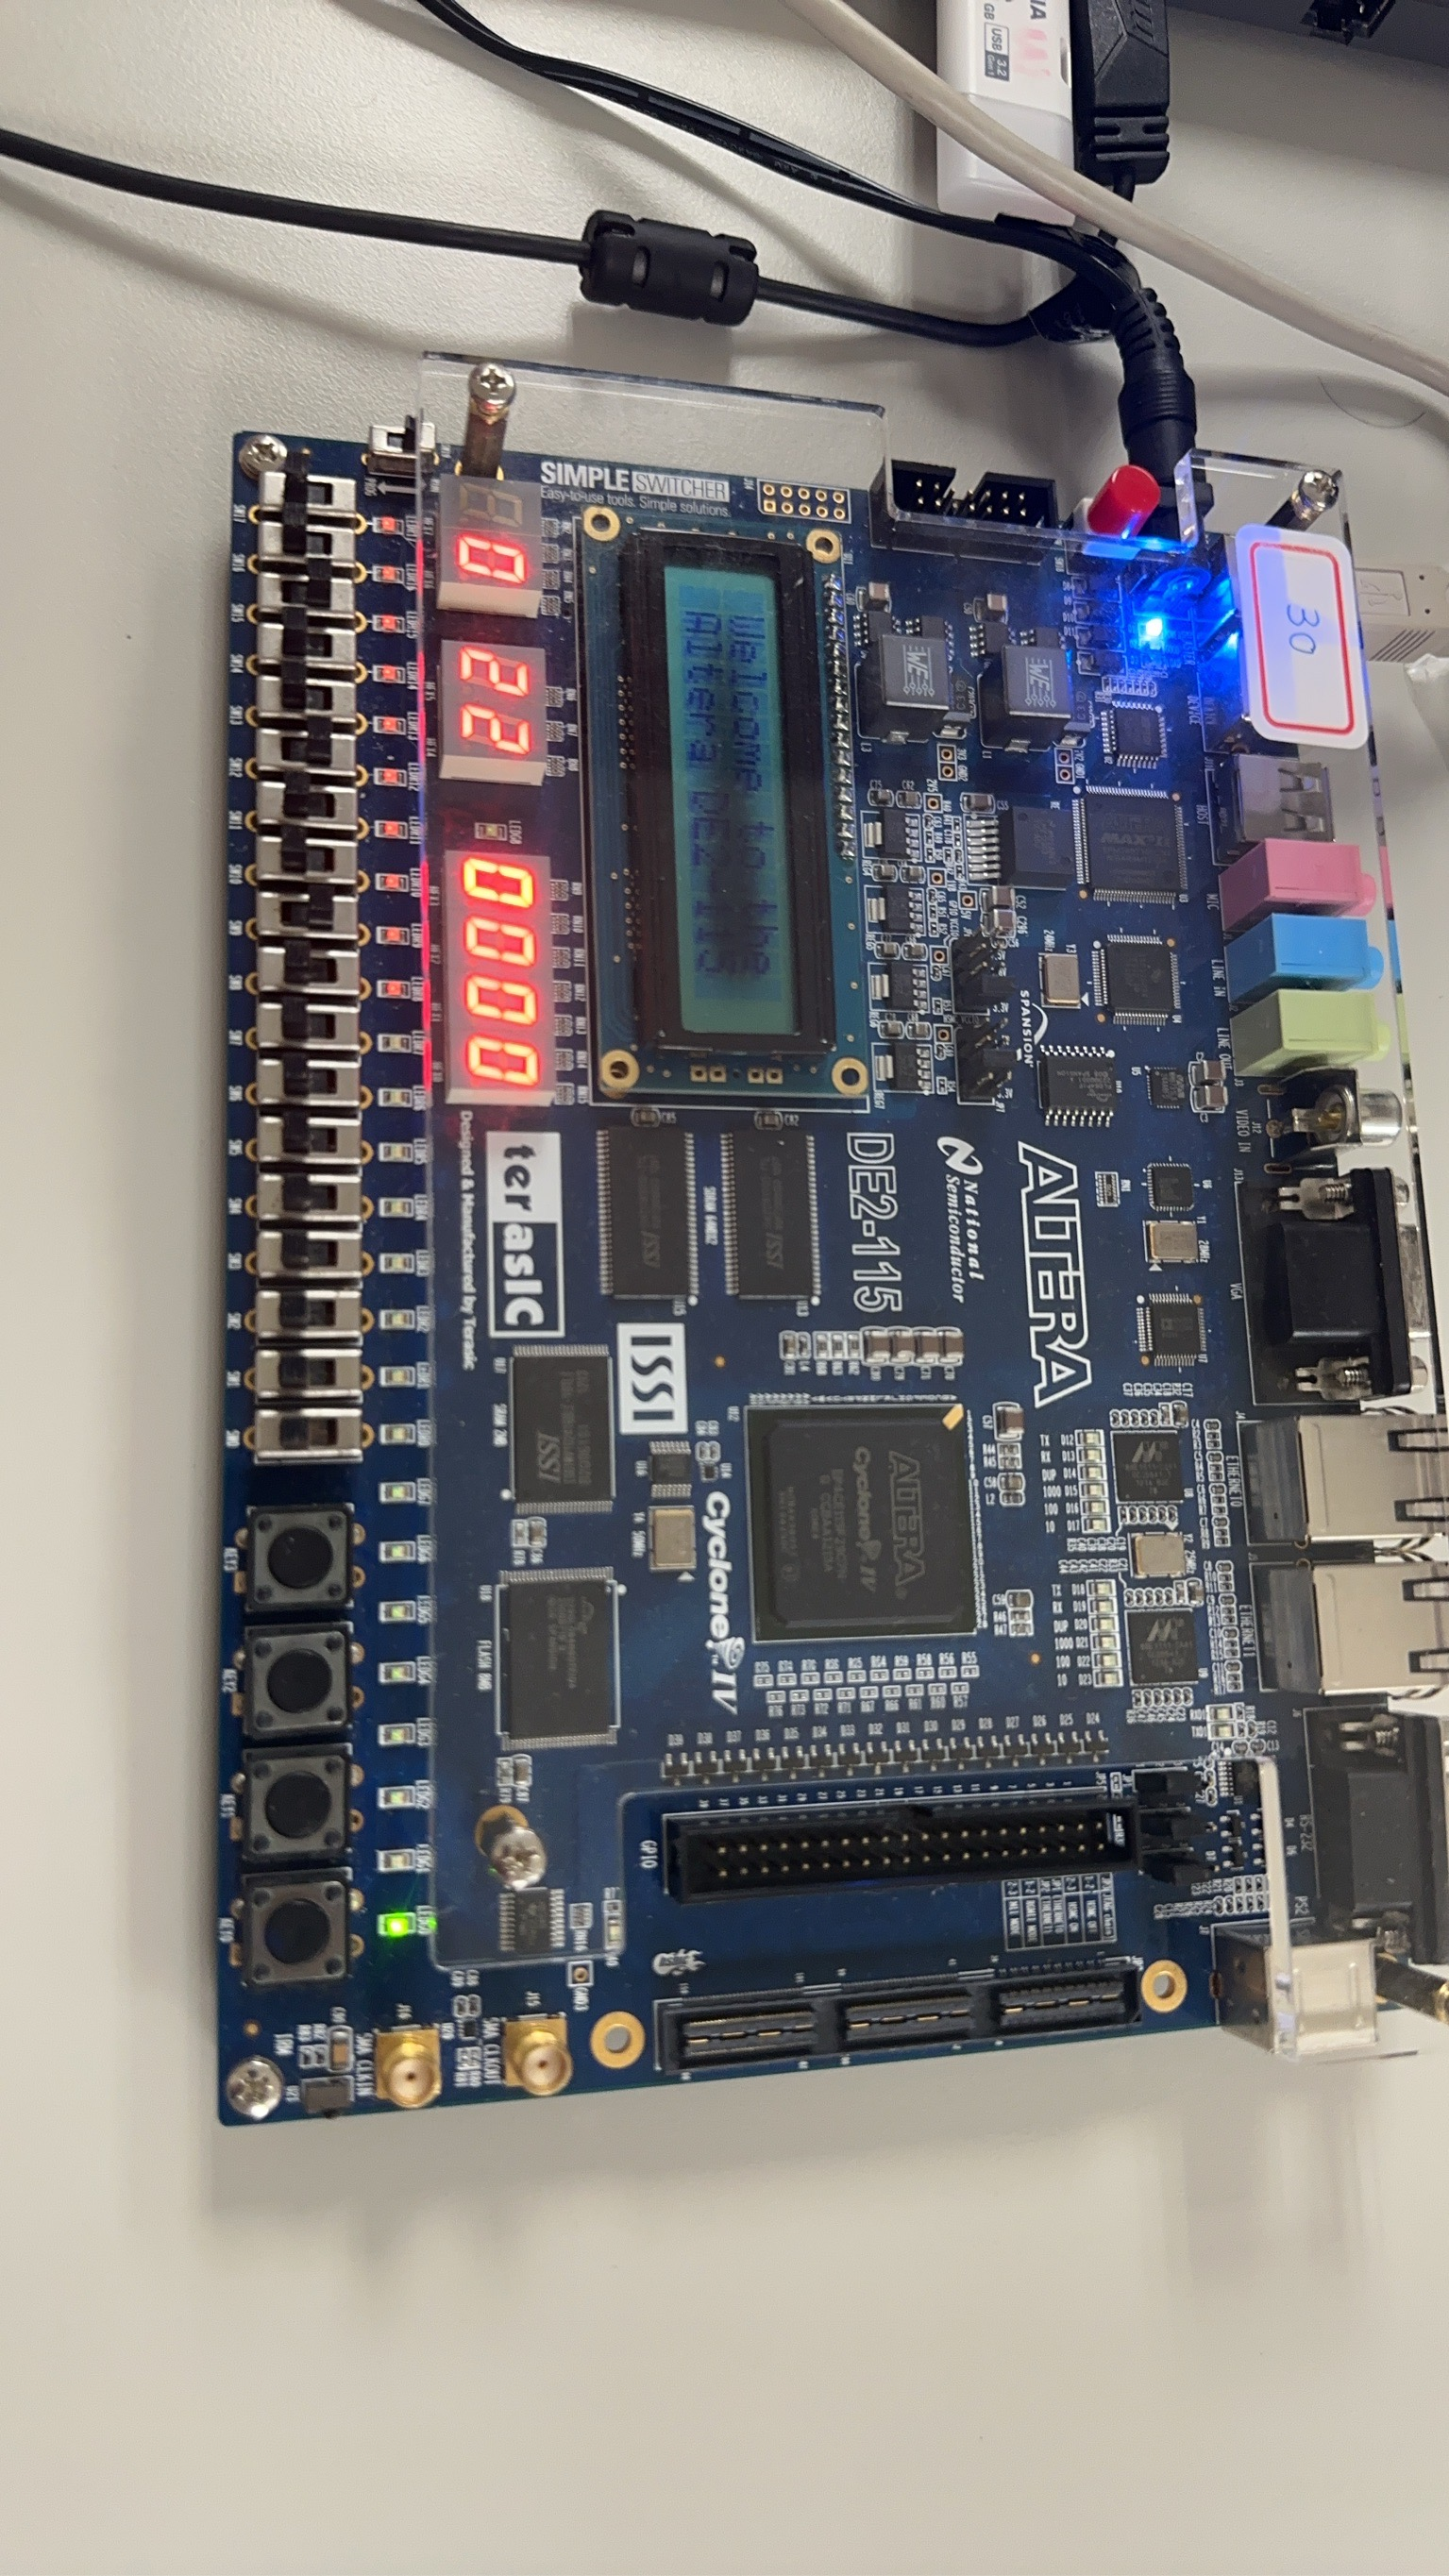
\includegraphics[width=\textwidth]{pipiline/demopicture/IMG_1155.jpeg}
        \caption{資料衝突前饋驗證狀態 (A)}
        \label{fig:forwarding_photo_1}
    \end{minipage}
    \hfill
    \begin{minipage}{0.48\textwidth}
        \centering
        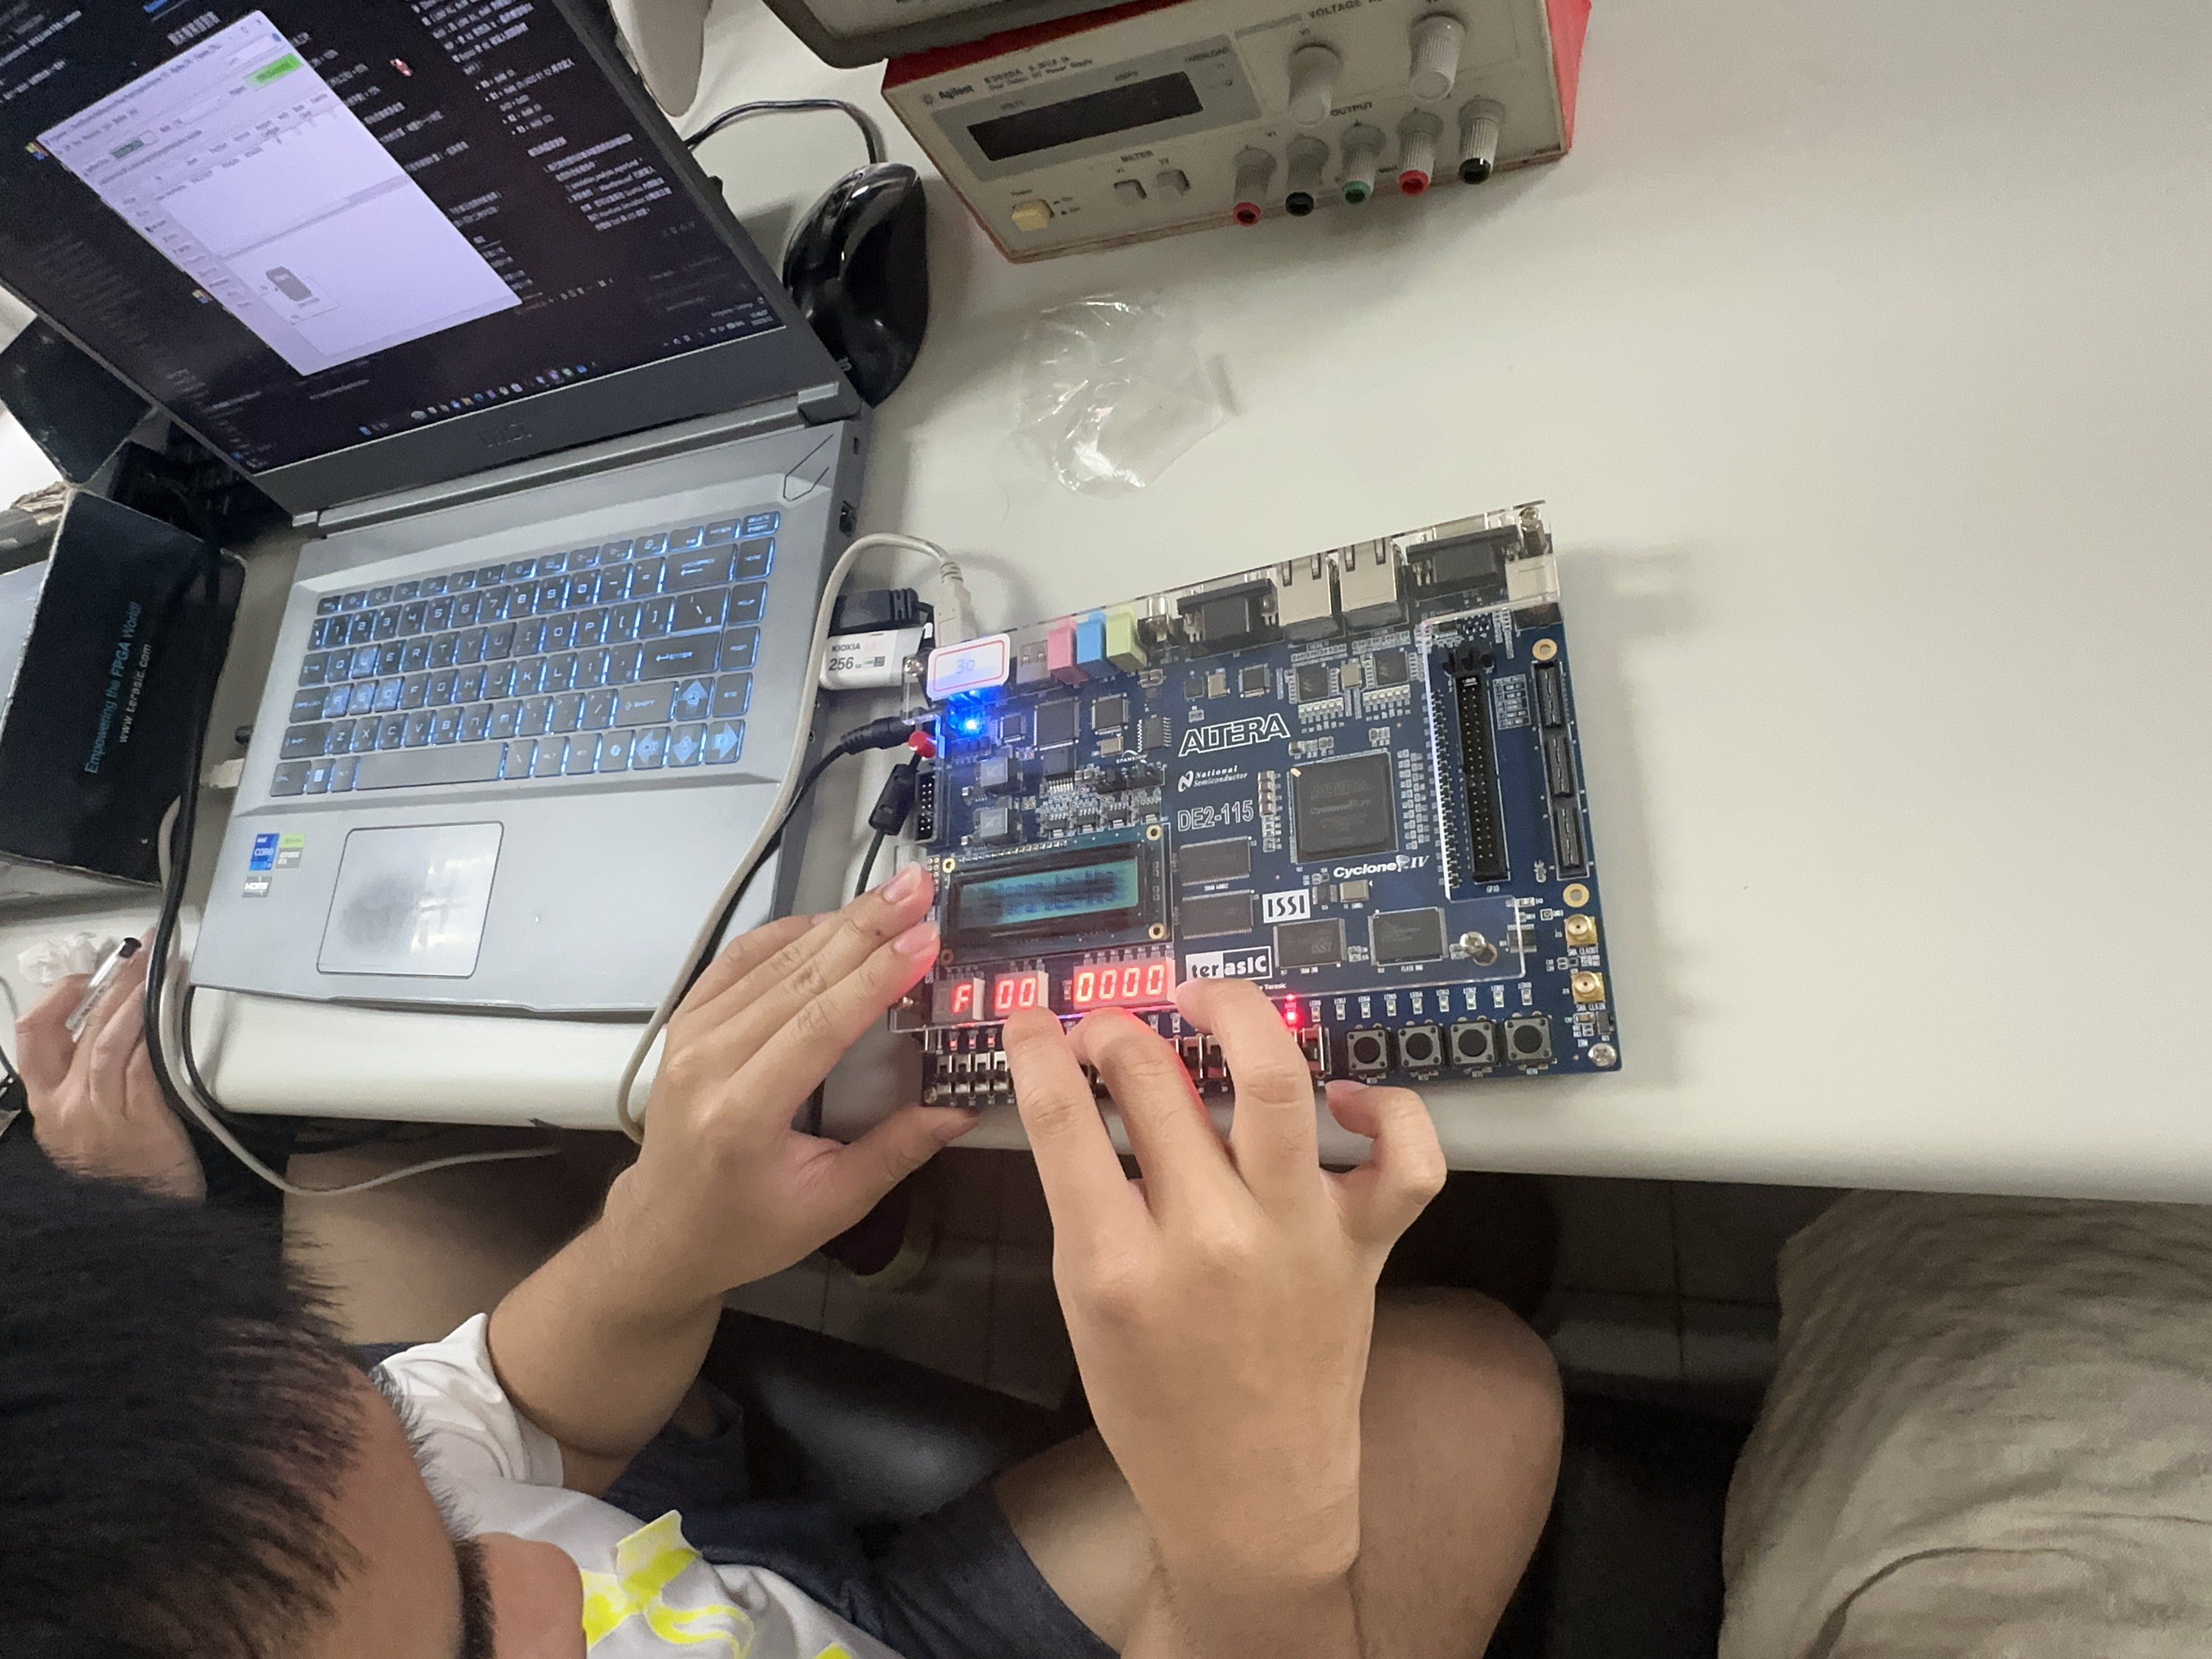
\includegraphics[width=\textwidth]{pipiline/demopicture/IMG_1157.jpeg}
        \caption{資料衝突前饋驗證狀態 (B)}
        \label{fig:forwarding_photo_2}
    \end{minipage}
\end{figure}

\begin{itemize}
    \item \textbf{IMG\_1156.jpeg}：展示了執行多時序除法 (DIV Stall) 時的硬體狀態。綠色 LED \texttt{LEDG[1]} (Exe Busy) 處於明亮狀態，表示管線目前被 DIV FSM 正確阻斷並暫停中。
\end{itemize}

\begin{figure}[H]
    \centering
    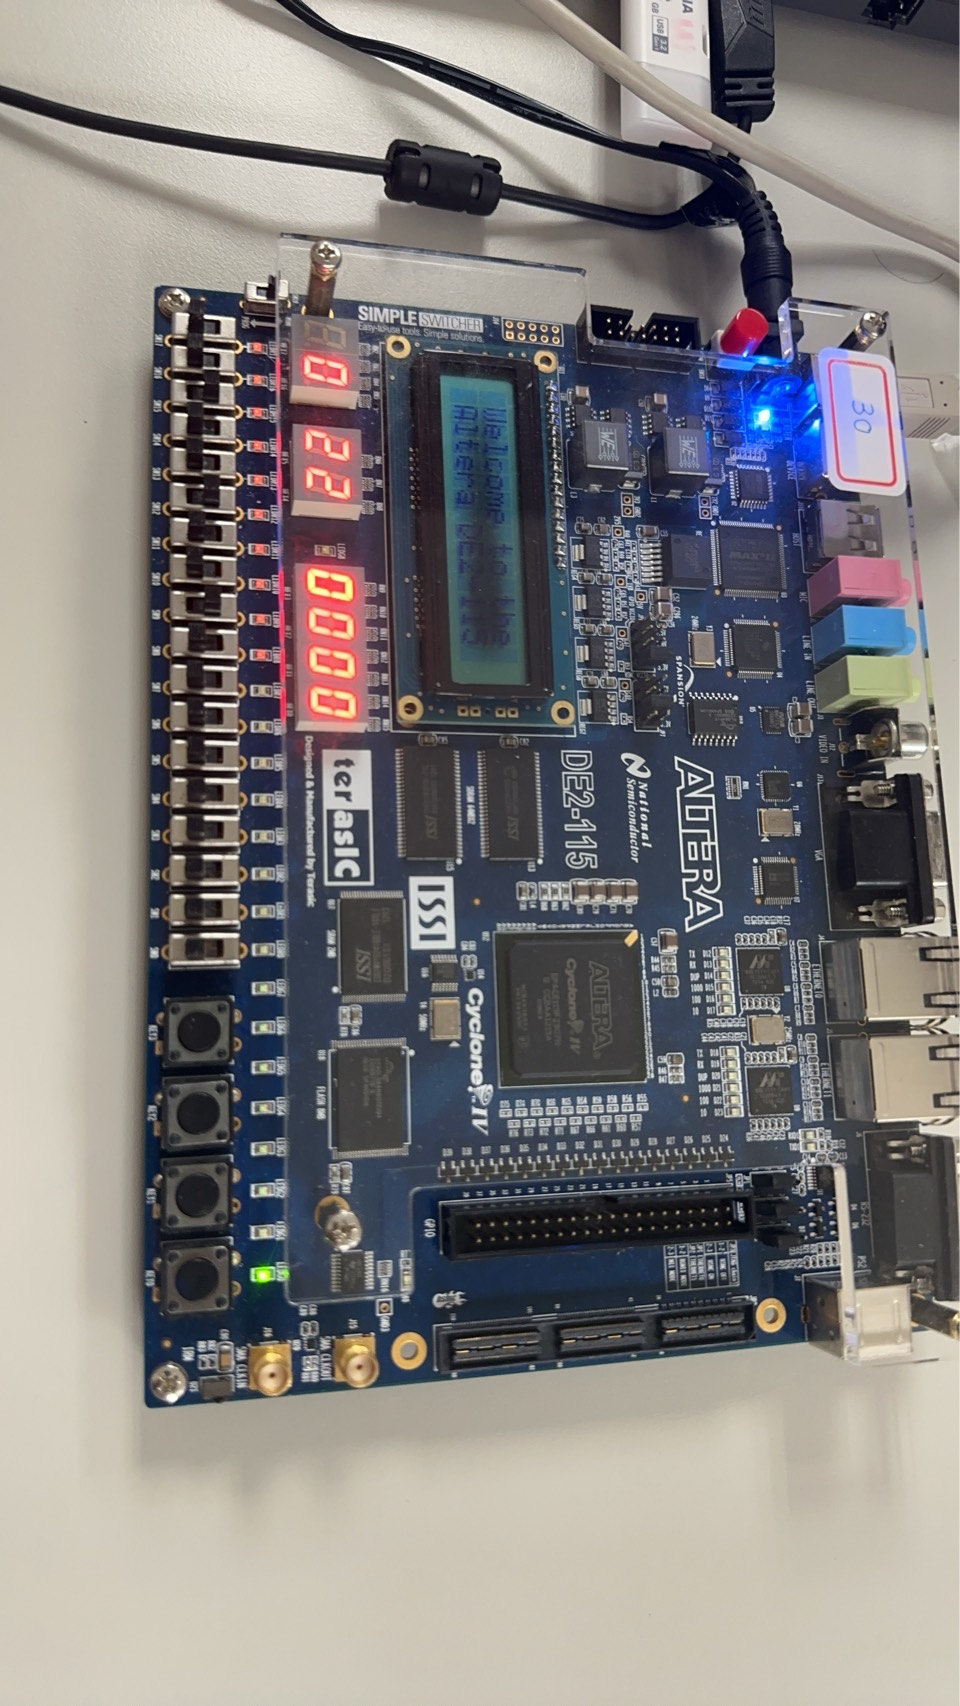
\includegraphics[width=0.6\textwidth]{pipiline/demopicture/IMG_1156.jpeg}
    \caption{多時序除法管線暫停 (DIV Stall) 驗證狀態}
    \label{fig:div_stall_photo}
\end{figure}

\begin{itemize}
    \item \textbf{IMG\_1158.mov}：錄製了手動時脈 \texttt{KEY[0]} 測試管線動作的動態影像，影片中流暢地示範了 5 組測資從撥碼開關設定、手動按鍵輸入，到暫存器數值與 Hazard LED 燈號即時閃爍變化的完整流動，確鑿證實了管線處理器具備高度穩定的硬體執行能力。
\end{itemize}

\section{實驗心得與深度思考}

\subsection{楊承諭的心得與思考 (微架構實作組)}

在這次期末專案中，將原本 Lab 9 的單週期（Single-cycle）多功能 CPU 重構為四階段管線（Pipeline）架構是一次極具挑戰性的過程。我面臨的第一個核心問題是\textbf{資料衝突（Data Hazard）與前饋（Forwarding）的時序對齊}。
在單週期處理器中，ALU 的輸出是在同一個時脈週期內直接鎖存回暫存器。然而在管線處理器中，當 \texttt{LOAD} 接著 \texttt{ADD} 執行時，\texttt{LOAD} 的結果要等到 WB 階段（第四個時脈）才會寫回暫存器檔案。如果我們不用 Stall 來暫停管線，就必須透過前饋多路選擇器（Mux）將資料「直接從流水線暫存器中拉回來」。

在除錯過程中，我曾遇到綠色 LED \texttt{LEDG[0]} (Hazard) 不正常持續發亮的問題。經過 Trace 程式碼發現，這是因為 \texttt{LOAD} 指令的 \texttt{Rs\_id}（作為寫入目標）與之前的空指令 \texttt{NOP} 產生了虛假比對。為此，我重寫了前饋判定邏輯，加入 \texttt{reads\_rs} 與 \texttt{reads\_rt} 這兩個控制訊號，明確區分出目前解碼的指令是否「確實需要讀取暫存器」，順利解決了這個 Bug。

另一個收穫是\textbf{多時序除法與管線暫停的融合}。實作移位相減除法器時，除法狀態機執行需要 8 個週期。如何在這 8 個時脈內「凍結」IF 與 ID 階段，同時讓 WB 階段正常流出，是我思考最久的部分。最終我採用了「氣泡插入（Bubbling）」技術：在 \texttt{stall = '1'} 時，強行將 \texttt{EXE/WB} 暫存器的 opcode 置為 \texttt{OP\_NOP} (1111)。這避免了當除法器在 EXE 階段計算時，WB 階段會重寫寫入先前暫存器資料的錯誤。這種軟硬體時序對齊的思維，讓我在實作中深刻體會到計算機組織（Computer Architecture）的奧妙。

\subsection{黃楷程的心得與思考 (驗證測試與報告組)}

我的主要工作是為這款四階段管線 CPU 設計具有高覆蓋率的測試資料，並在板子上進行實體操作與拍照錄影。在設計測資時，我必須細緻地考慮到\textbf{管線深度對時序的影響}。

例如在測資 1（無 Hazard 基本運算）中，為了讓同學與助教能清晰觀察到 \texttt{LOAD R1, 5} 和 \texttt{LOAD R2, 7} 真正寫入暫存器陣列，我必須在它們後面手動插入兩個 \texttt{NOP}。這是因為在四階段管線中，指令從讀入指撥開關（IF）到真正寫回暫存器檔案（WB）需要經歷 3 個 Clock 的延遲。如果不插入 NOP，暫存器顯示器就不會即時顯示出 \texttt{05} 和 \texttt{07}。

此外，在驗證多時序除法（測資 4）時，我們必須手動按壓 \texttt{KEY[0]} 鍵 8 次來提供時脈。我們發現在這 8 次按壓中，左側顯示 IF/ID 的七段顯示器 \texttt{HEX4} 和 ID/EXE 的 \texttt{HEX6} 真的像被「凍結」一樣， opcode 牢牢固定在除法的 \texttt{8} 上，同時 \texttt{LEDG[1]} 保持明亮。這種親眼看見硬體電路按照我們設計的狀態機暫停、插氣泡、計算，最後在第 8 個 Clock 結束瞬間「答！」一聲解鎖並讓管線重新流動的過程，給了我極大的震撼。這比單純在 ModelSim 上看波形圖更具實體感，也讓我更敬佩硬體工程師在細節處理上的嚴謹性。

\section{小組工作分配與貢獻度}

本小組兩位成員分工明確，緊密配合，實現了高效率開發與高質量報告撰寫：

\begin{table}[H]
    \centering
    \caption{組員分工與貢獻度表}
    \label{tab:contributions}
    \begin{tabular}{@{}llcp{8.5cm}@{}}
        \toprule
        \textbf{學號} & \textbf{姓名} & \textbf{比重} & \textbf{具體負責工作內容描述} \\ \midrule
        \texttt{113590051} & 楊承諭 & \textbf{50\%} & 
        1. 負責\href{file:///home/chengyu/\%E6%A1%8C%E9%9D%A2/Microcomputer_System/Finial_Project/pipiline/Pipeline_CPU.vhd}{Pipeline\_CPU.vhd} 的整體架構設計。\\
        & & & 2. 實作 IF/ID, ID/EXE, EXE/WB 等管線暫存器與資料通路。\\
        & & & 3. 設計 Data Forwarding Unit（前饋單元）解決 EXE 與 WB 資料衝突。\\
        & & & 4. 撰寫多時序移位相減除法器狀態機與管線凍結、氣泡插入（Stall \& Bubble）邏輯。\\
        & & & 5. 處理除以零 Bypass 等防錯功能與 Quartus II 編譯除錯。\\ \midrule
        \texttt{113590017} & 黃楷程 & \textbf{50\%} & 
        1. 負責\href{file:///home/chengyu/\%E6%A1%8C%E9%9D%A2/Microcomputer_System/Finial_Project/cpu_test_data_suite.md}{cpu\_test\_data\_suite.md} 5組測試資料的邏輯時序設計。\\
        & & & 2. 於 DE2-115 開發板上進行 5 組測資的手動輸入與實體驗證操作。\\
        & & & 3. 拍攝實驗驗證所需的照片與演示影片，記錄硬體正確顯示狀態。\\
        & & & 4. 協助編寫期末專案簡報，並負責彙整小組心得與最終書面報告。\\ \bottomrule
    \end{tabular}
\end{table}

\end{document}
